\section { Parameterization of the Detector Response}


Published are the measured data. To compare them to the model predictions,
one needs to know how the theoretical spectrum is modified by the detector
response, i.e. know the detector response.

Fortunately, references  \cite{RMC_1992_PhysRevC.46.1094}, \cite{RMC_1999_PhysRevC.59.2853}
have the detector response published.

Also published is the RPC spectrum on $H_2$ used for calibration.

We check how well different parameterizations of the detector response describe the
calibration peak.
\begin{figure}[htbp]
 \begin{center}
 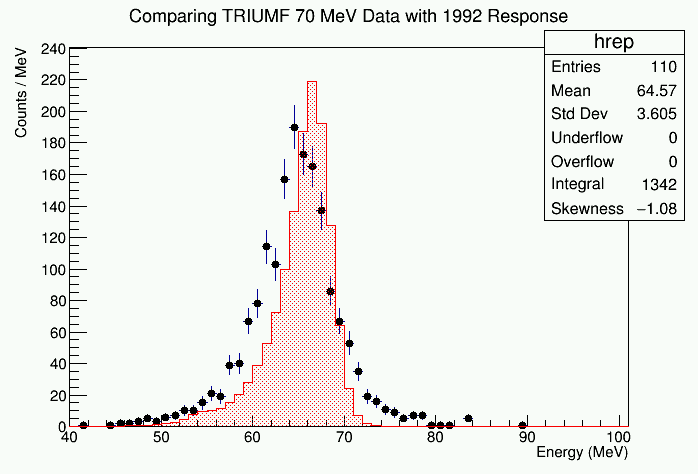
\includegraphics[width=0.49\columnwidth]{png/70MeV_vs_1992_Response} 
 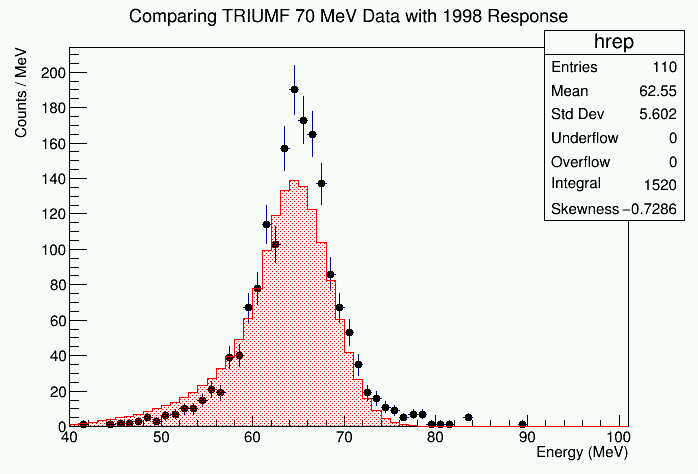
\includegraphics[width=0.49\columnwidth]{png/70MeV_vs_1998_Response} 
 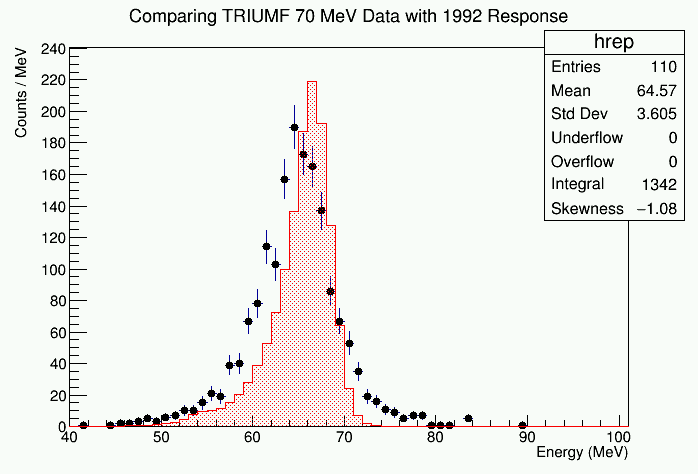
\includegraphics[width=0.49\columnwidth]{png/70MeV_vs_1992_Response} 
 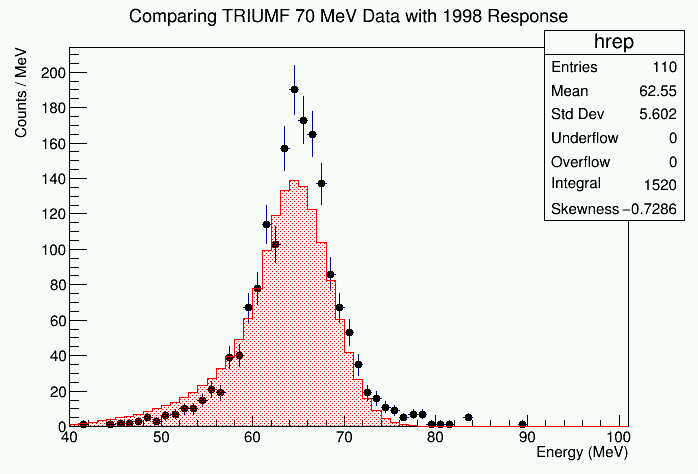
\includegraphics[width=0.49\columnwidth]{png/70MeV_vs_1998_Response} 
 \end{center}
 \caption{\red{ \bf Caption}}
 \label{p004}
 \end{figure}
